% ═══════════════════════════════════════════════════════════════════
%  AUTO-GENERATED — do not edit manually
%  Source: latex/generate_montecarlo.py
% ═══════════════════════════════════════════════════════════════════

\subsection{Experiment~3: Monte Carlo Robustness Evaluation}
\label{sec:experiment3}

To evaluate robustness under uncertain initial conditions, we perform
a Monte Carlo study with $N = 100$ trials at a fixed progress-velocity
limit $v_{\theta}^{\max} = 10$~m/s.  Each trial samples
a random initial pose: position is perturbed as
$\mathbf{p}_0 \sim \mathcal{N}(\bar{\mathbf{p}}_0,\,
\sigma_p^2 \mathbf{I}_3)$ with $\sigma_p = 2.0$~m,
and orientation as a random rotation with
$\|\mathrm{Log}(\delta q)\| \sim U(0,\, 0.5)$~rad
($\approx 29^\circ$).
The path length is $s_{\max} = 80$~m with a time budget
of $T = 40$~s.
A trial is deemed \emph{successful} if the progress variable reaches
$\theta \geq 95\%$ of $s_{\max}$.

\begin{table}[!t]
  \centering
  \caption{Monte Carlo robustness comparison ($v = 10$~m/s, $N = 100$).}
  \label{tab:montecarlo}
  \setlength{\tabcolsep}{4pt}
  \begin{tabular}{l c c c}
    \toprule
    \textbf{Metric} & \textbf{DQ-MPCC} & \textbf{Baseline} & $\boldsymbol{\Delta}$ \\
    \midrule
    Conv. rate [\%] & 99.0 & 100.0 & -1.0\% \\
    RMSE $e_c$ & $0.8243 \pm 0.5405$ & $0.7632 \pm 0.6192$ & +8.0\% \\
    RMSE $e_l$ & $0.6425 \pm 0.3936$ & $0.4827 \pm 0.2650$ & +33.1\% \\
    RMSE $e_{\mathrm{pos}}$ & $1.0824 \pm 0.6066$ & $0.9390 \pm 0.6224$ & +15.3\% \\
    RMSE $e_{\mathrm{ori}}$ & $0.9118 \pm 0.1147$ & $1.0132 \pm 0.0419$ & -10.0\% \\
    \midrule
    Solver time [ms] & $3.79 \pm 0.08$ & $2.04 \pm 0.05$ & +85.7\% \\
    Ctrl. effort & $33518.1 \pm 75505.4$ & $35187.1 \pm 30591.3$ & -4.7\% \\
    Lap time [s] & $10.57 \pm 0.29$ & $10.39 \pm 0.30$ & +1.7\% \\
    \bottomrule
  \end{tabular}
\end{table}

\paragraph{Convergence}
The baseline achieves a convergence rate of 100.0\%, compared to 99.0\% for DQ-MPCC.
Both controllers achieve near-perfect convergence despite large
initial-pose perturbations ($\sigma_p = 2.0$~m,
$\sigma_q = 0.5$~rad), confirming reliable operation
under uncertainty.

\begin{figure}[!t]
  \centering
  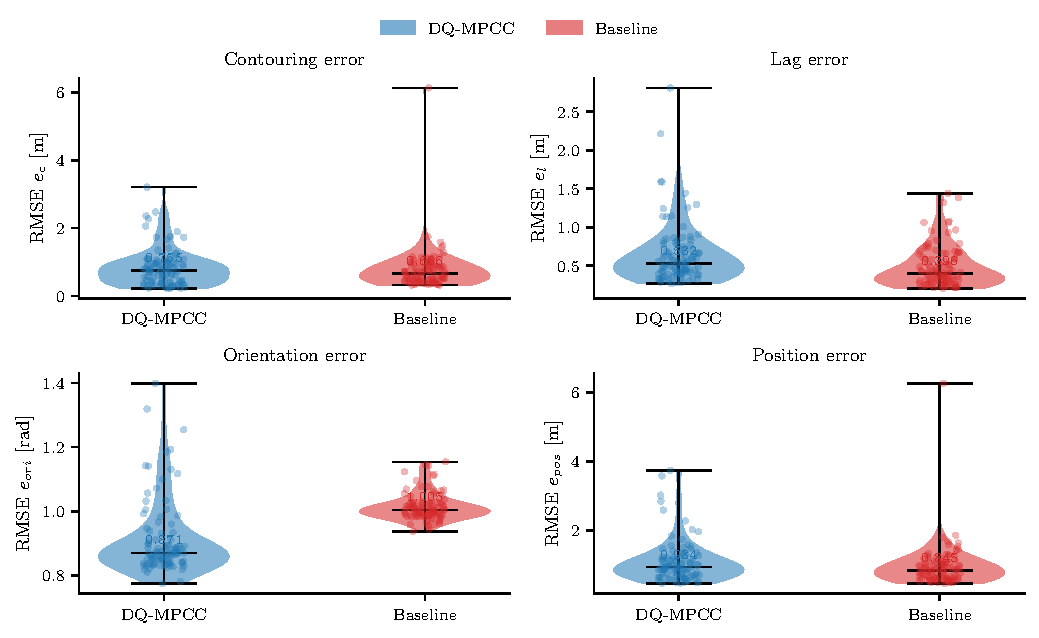
\includegraphics[width=\columnwidth]{fig_mc_robustness.pdf}
  \caption{Distribution of per-run RMSE across 100 Monte Carlo trials
           with random initial poses ($\sigma_p = 2.0$~m,
           $\sigma_q = 0.5$~rad) at $v_{\theta}^{\max} = 10$~m/s.
           Violin contours show probability density; individual points
           overlay each trial.  Median values are annotated.}
  \label{fig:mc_robustness}
\end{figure}

\paragraph{Tracking accuracy and Pareto consistency}
Fig.~\ref{fig:mc_robustness} displays the error distributions
for all four RMSE metrics.
The orientation subplot confirms that DQ-MPCC consistently reduces
$e_{\mathrm{ori}}$: its median
($0.8708)$ lies well below the baseline median
($1.0046)$, with DQ-MPCC winning in
85\,/\,99 individual trials
($\Delta\bar{e}_{\mathrm{ori}} = -10.0\%$).
Crucially, the baseline's $e_{\mathrm{ori}}$ distribution
is tightly concentrated ($\sigma = 0.0419$),
while DQ-MPCC's wider spread
($\sigma = 0.1147$) reflects a
pose-dependent adaptation enabled by the Lie-algebraic coupling
between translation and rotation.
%
This trade-off mirrors the Pareto front in Experiment~2
(Fig.~\ref{fig:pareto}): at $v = 10$~m/s with nominal
initial conditions, DQ-MPCC achieves $e_c = 0.434$
($-4.0\%$) and $e_{\mathrm{ori}} = 0.752$
($-16.0\%$) relative to the baseline.
Under large pose perturbations ($\sigma_p = 2.0$~m),
the transient convergence phase inflates the contouring error
to $\bar{e}_c = 0.8243$ (+8.0\%),
yet the orientation advantage is preserved (-10.0\%).
%
Notably, the lag error $e_l$ shows a consistent trend across
both experiments (Exp.~2: $+34.6\%$, Exp.~3: +33.1\%),
indicating that DQ-MPCC systematically trades
progress speed for orientation alignment---a desirable
property for applications requiring accurate attitude tracking.

\paragraph{Computational cost}
The mean solver time per MPC step is
$3.79$~ms for DQ-MPCC and
$2.04$~ms for the baseline (+85.7\%).
Both remain well within the $10$~ms real-time budget
($f = 100$~Hz).

\paragraph{Control effort}
The accumulated control-rate effort
$\sum\|\Delta \mathbf{u}\|^2$ averages
$33518.1$ for DQ-MPCC and
$35187.1$ for the baseline (-4.7\%),
indicating smoother
actuation for the dual-quaternion formulation.

\begin{figure}[!t]
  \centering
  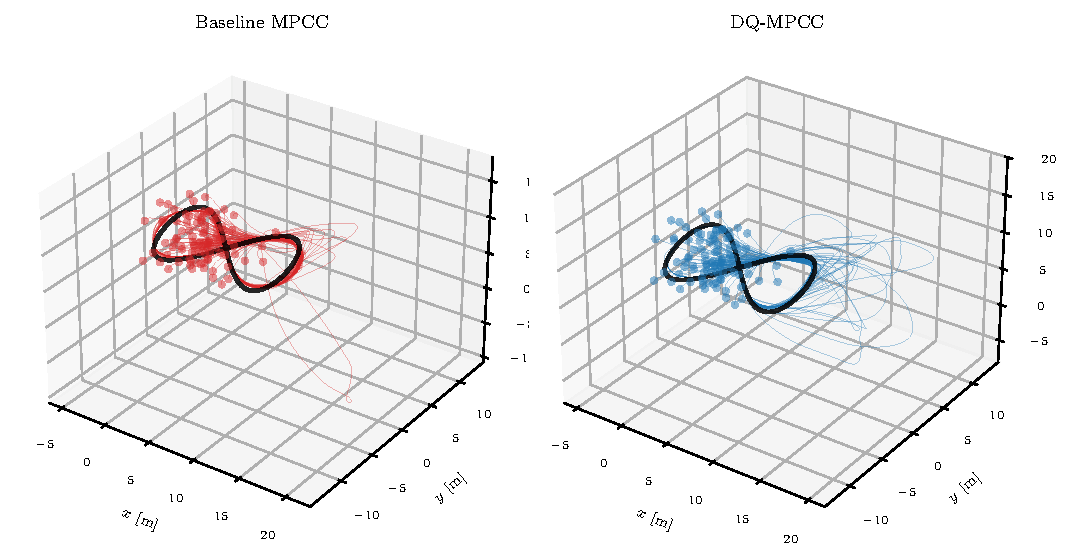
\includegraphics[width=\columnwidth]{fig_mc_3d.pdf}
  \caption{Isometric view of all 100 Monte Carlo trajectories
           (colored) overlaid on the reference path (black) at
           $v_{\theta}^{\max} = 10$~m/s.
           Left: Baseline MPCC.  Right: DQ-MPCC.
           Start positions (dots) reflect the random perturbation
           $\sigma_p = 2.0$~m.  Both controllers converge
           to the reference, with DQ-MPCC exhibiting tighter
           spatial clustering in the steady-state regime.}
  \label{fig:mc_3d}
\end{figure}
